\documentclass[11pt,a4paper]{article}

\usepackage[utf8]{inputenc} 
\usepackage[T1]{fontenc} 
\usepackage{lmodern}
\usepackage[margin=2cm]{geometry}
\usepackage[german]{babel}
\usepackage{amsmath} 
\usepackage{graphicx} 
\usepackage{booktabs}
\usepackage{hyperref}
\usepackage{breqn}
\hypersetup{
    colorlinks,
    citecolor=red,
    filecolor=black,
    linkcolor=black!20!blue!90!,
    urlcolor=black} 
\usepackage{nicefrac}
\usepackage[table]{xcolor}
\usepackage{tocloft}
\usepackage{multirow}

\setlength{\parindent}{0pt}
\setlength{\parskip}{1ex plus 0.5ex minus 0.5ex}

\definecolor{incolor}{rgb}{0.0, 0.0, 0.5}

\hbadness=99999

\newcommand{\refpy}[1]{Siehe Anhang: \textit{Rechnungen in Python} (\texttt{{\color{incolor}In [{\color{incolor}#1}]}})}
\newcommand\dif{\mathop{}\!\mathrm{d}}
\newcommand\vphi{\varphi}
\newcommand\mean{\begin{equation}
\frac{\sum_{i=1}^n I_{V_i}}{n}\label{mean}
\end{equation}}
\newcommand\meanstd{\begin{equation}
s_x=\sqrt{\frac{1}{n-1}\sum_{i=1}^n(x_i-\overline{x})^2}\label{meanstd}
\end{equation}}
\newcommand\prodquo{\begin{equation}\left\vert\frac{\Delta z}{z}\right\vert=\sqrt{\left(a\frac{\Delta x}{x}\right)^2+\left(b\frac{\Delta y}{y}\right)^2+\ldots}\textrm{ f\"ur }z=x^a\ y^b\ldots\end{equation}}
\newcommand{\halftime}[4]{\begin{figure}[h]
\begin{minipage}{.#1\textwidth}#3\end{minipage}\begin{minipage}{.#2\textwidth}
\centering
#4\end{minipage}
\end{figure}}


\begin{document}

{
\centering 
\large 
Physiklabor für Anf\"anger*innen \\
Ferienpraktikum im Sommersemester 2018 \\[4mm]
\textbf{\LARGE 
Versuch 19: Gekoppeltes Pendel 
} \\[3mm]
(durchgef\"uhrt am 19.09.2018 bei Adrian Hauber) \\
Gruppe 14: Andréz Gockel, Patrick M\"unnich\\
\today \\[10mm]
}

\vspace{50pt}
\tableofcontents
\vspace{22pt}
\listoftables
\vspace{22pt}
\listoffigures
\pagebreak

\section{Ziel des Versuchs}
Das Ziel dieses Versuchs ist einen gekoppelten Oszillator durch einen gekoppelten Pendel zu veranschaulichen. Hierzu werden erst die Differentialgleichungen hergeleitet und durch das Drehmoment entkoppelt, um die Eigenfrequenzen zu berechnen womit die Schwebungsdauer aus den Schwingungsdauern berechnet werden kann. In diesem Versuch werden Periodendauern bei verschiedenen Kopplungsgraden gemißt und zusätzlich die Schwebungsdauer. Der Kopplungsgrad wird verändert indem die Kopplungsfeder verschoben wird. Zusätzlich wird der Koppelungsgrad durch die Schwingdauern berechnet.

\section{Messung der Schwingungsdauern}

\subsection{Theorie}

Um den Koppelungsgrad zu bestimmen wird zunächst die Differentialgleichung des gekoppelten Pendels hergeleitet.

Wir beginnen dazu mit dem r\"ucktreibenden Moment infolge der Schwerkraft bei kleinen Auslenkungen $\vphi$:
\begin{equation}
M=-mgl\vphi=D_g\vphi\label{M1}
\end{equation}
Dazu gibt es bei jedem Pendel ein Kopplungsmoment $D_f(\vphi_2-\vphi_1)$. Es existiert noch ein weiteres Moment, welches von der Vorspannung der Feder her r\"uhrt. Dieses gibt es, da die Feder schon wenn die Pendel in paralleler Lage stehen eine gewisse Spannung besitzt. Beide Pendel weisen in der Ruhelage einen Ausschlag $\alpha$ bzw. $-\alpha$ in Bezug auf die Vertikallage auf. Wenn man aber die Auslenkungen $\vphi_1$ und $\vphi_2$ von der Gleichgeweichtslage aus rechnet, so f\"allt dieses Moment aus der Rechnung raus, da es durch ein Moment $mgl\pm\alpha$ kompensiert wird. Wir erhalten also als Momentengleichungen:
\begin{align}
\begin{split}
{M_1=-D_g\vphi_1+D_f(\vphi_2-\vphi_1)}
\\
{M_2=-D_g\vphi_2-D_f(\vphi_2-\vphi_1)}
\end{split}
\end{align}
Setzen wir diese in die Bewegungsgleichung eines physikalischen Pendels 
\[
I\ddot{\vphi}=M=-mgl\sin\vphi
\]
ein, so erhalten wir 
\begin{align}
\begin{split}
{I\frac{\dif^2\vphi_1}{\dif t^2}=-D_g\vphi_1+D_f(\vphi_2-\vphi_1)}
\\
{I\frac{\dif^2\vphi_2}{\dif t^2}=-D_g\vphi_2-D_f(\vphi_2-\vphi_1).}
\end{split}
\end{align}
Addieren bzw. subtrahiert man die Differentialgleichungen f\"ur die Winkelsumme $(\vphi_2+\vphi_1)$ bzw. die Winkeldifferenz $(\vphi_2-\vphi_1)$, so liefert dies:
\begin{align}
\begin{split}
{I\frac{\dif^2(\vphi_2+\vphi_1)}{\dif t^2}=-D_g(\vphi_2+\vphi_1)}\\
{I\frac{\dif^2(\vphi_2-\vphi_1)}{\dif t^2}=-(D_g+2D_f)(\vphi_2-\vphi_1)}
\end{split}
\end{align}
Nutzt man hierauf den L\"osungsansatz
\begin{align}
\begin{split}
{(\vphi_2+\vphi_1)=2A\cos(\omega t+\delta)}\\
{(\vphi_2-\vphi_1)=2B\cos(\Omega t+\Delta),}
\end{split}
\end{align}
so erh\"alt man die Kreisfrequenzen
\begin{equation}
\omega=\sqrt{\frac{D_g}{I}}\textrm{   und   }\Omega=\sqrt{\frac{D_g+2D_f}{I}}
\end{equation}
Mit $I=mr^2$, hier ist $r$ der Abstand $L$ zwischen Masse und Rotationsachse, und (\ref{M1}) kommen wir also auf:
\begin{equation}
\omega=\sqrt{\frac{g}{L}}\textrm{   und   }\Omega=\sqrt{\frac{g}{L}-\frac{2D_fl^2}{mL^2}}
\end{equation}
Dies sind die Kreisfrequenzen f\"ur gleich- und gegensinnige Schwingung.

Wichtig ist f\"ur diesen Versuch noch die Gleichung f\"ur den Kopplungsgrad,
\begin{equation}
	K=\frac{T_B^2-T_A^2}{T_B^2+T_A^2}
\end{equation}

\subsection{Aufbau}

\halftime{5}{5}{In diesem Versuch haben wir zwei Pendel mit die aus einer festen Stange und einem Zusatzkörper bestehen. Eine Feder die beide Pendel koppelt hängt mit der verstellbaren Länge $l$ von dem Aufhängepunkt des Pendels. Vor beginn der Messungen ist zu beachten:
\begin{itemize}
	\item das der Aufbau komplett eben sein muss
	\item das beide Pendel mit gleicher Periodendauer schwingen
\end{itemize}
Unsere Kalibriermessung ergab $18.70(5)$\,s für 10 Schwingungen beider Pendel. % maybe formulate gooder
Die länge der Pendel von Aufhängepunkt zu der Masse ist jeweils $L = 95.0(5)$\,cm.
}{\fbox{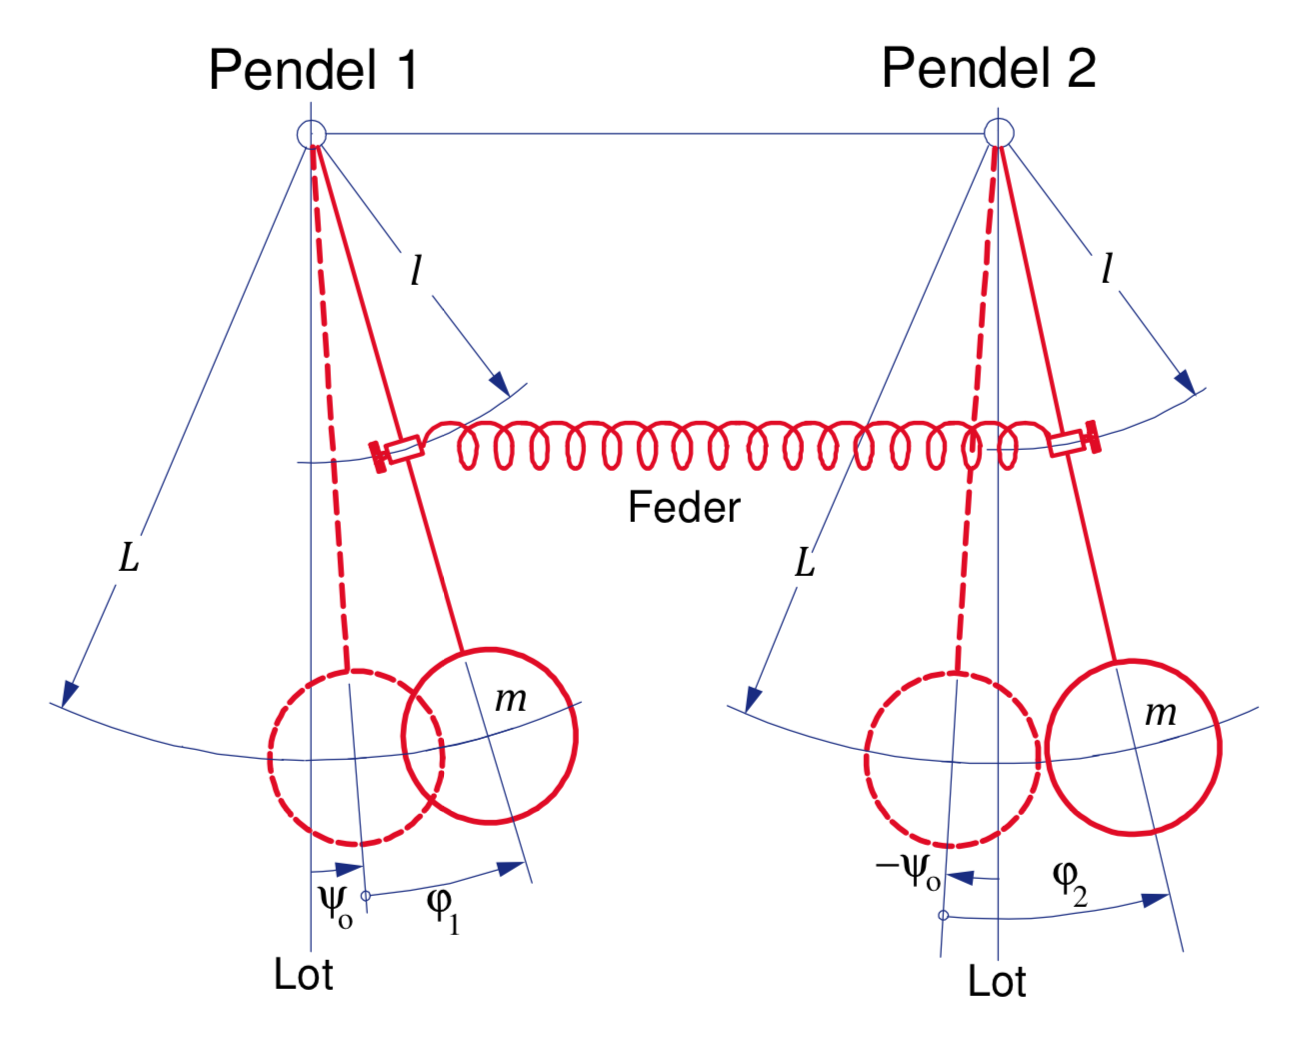
\includegraphics[width=0.9\textwidth]{ndp}}
   \renewcommand\thefigure{B1}
\caption[Gekoppeltes Pendel]{Gekoppeltes Pendel \cite{Anleitung}}
\label{Pic:1}}

\subsection{Durchführung}

Zuerst haben wir die Periodendauer f\"ur 20 Schwingungen bei gegen- und gleichsinniger Schwingung gemessen. Daraufhin die Schwingungsdauer f\"ur Schwebung. In unserem Fall wurde nicht beachtet, dass die Schwingungsdauer die doppelte Zeit zwischen zwei Stillst\"anden des gleichen Pendels ist. 

Nachdem diese Werte gemessen wurden, wurde dies mit insgesamt drei anderen Kopplungsst\"arken nochmals durchgef\"uhrt. Hierzu wird die Kopplungsfeder einfach nach oben bzw. nach unten verschoben. Hierbei wichtig war, dass die Kopplung nicht zu stark sein sollte.

Wir erhalten also vier Messreihen, aus denen wir dann unsere Kopplungsgrade berechnen und die gemessenen und berechneten Werte f\"ur die Periodendauer der Schwebung vergleichen.

\pagebreak

\subsection{Auswertung}

Wir beginnen damit, dass wir von unseren Messwerten die Mittelwerte von den Periodendauern f\"ur jeweils gleichsinnige, gegensinnige, und schwebende Schwingungen berechnen. Die Rechnung hierf\"ur folgt \"uber die allgemeinen Formeln f\"ur die Berechnung von Mittelwerten und dessen Fehler:
\mean
\meanstd
Diese Werte werden dann f\"ur die Berechnung unseres Kopplungsgrades genutzt. Die Formel f\"ur den Kopplungsgrad ist von $T_A$, der Periodendauer f\"ur entgegengesetzte Schwingung, und $T_B$, der Periodendauer f\"ur gleichsinnige Schwingung, abh\"angig, welche beide einen Fehler beinhalten. Zur Fehlerberechnung benutzen wir die Gau\ss sche Fehlerfortpflanzung.
Wir leiten also einmal partiell nach $T_A$ und einmal nach $T_B$ ab:
\[
	\frac{\partial K}{\partial T_A}=-\frac{4T_AT_B^2}{(T_A^2+T_B^2)^2}
\]
\[
	\frac{\partial K}{\partial T_B}=\frac{4T_A^2T_B}{(T_B^2+T_B^2)^2}
\]
Daraus erhalten wir als Unsicherheiten von K:
\begin{equation}
	\Delta K=\sqrt{\left(\Delta T_A\frac{\partial K}{\partial T_A}\right)^2+\left(\Delta T_B\frac{\partial K}{\partial T_B}\right)^2}
\end{equation}

Um die Periodendauer der Schwebung zu berechnen nutzen wir die folgende Funktion:
\begin{equation}
	T_S=2\frac{T_AT_B}{T_B-T_A}
\end{equation}
Wir k\"onnen wieder gleich wie zuvor die Formel f\"ur Quotienten verwenden und erhalten als Ableitungen:
\[
	\frac{\partial T_S}{\partial T_A}=2\frac{T_B^2}{(T_A-T_B)^2}
\]
\[
	\frac{\partial T_S}{\partial T_B}=-2\frac{T_A^2}{(T_B-T_A)^2}
\]
Die Unsicherheit von $T_S$ setzt sich dann auch wie zuvor folgenderma\ss en zusammen:
\begin{equation}
	\Delta T_S=\sqrt{\left(\Delta T_A\frac{\partial T_S}{\partial T_A}\right)^2+\left(\Delta T_A\frac{\partial T_S}{\partial T_A}\right)^2}
\end{equation}

\pagebreak

Wir erhalten aus diesen Rechnungen f\"ur $K$:
\begin{itemize}
	\item $0.112\pm0.008$
	\item $0.160\pm0.010$
	\item $0.036\pm0.008$
	\item $0.229\pm0.009$
\end{itemize}

F\"ur $T_S$ dann:
\begin{itemize}
	\item $31\pm2.4$
	\item $21\pm1.3$
	\item $100\pm23$
	\item $15.9\pm0.4$
\end{itemize}

Berechnete Werte f\"ur $T_S$ lauten:
\begin{itemize}
	\item $30.9\pm0.4$
	\item $20.6\pm0.4$
	\item $98.0\pm0.4$
	\item $15.9\pm0.4$
\end{itemize}


\section{Diskussion}

Betrachten wir erstmal unsere berechneten und gemessenen Werte f\"ur die Periodendauer von Schwebung:\\
Beim ersten Blick auf die Werte f\"allt klar auf, dass die dritte Periodendauer einen sehr gro\ss en Fehler besitzt. Dies stammt daraus, dass die Differenz der Frequenzen von der gleich- und gegensinnigen Schwingungen sehr klein sind. Betrachten wir wieder unsere Formel f\"ur $T_S$, so sehen wir, dass der Fehler sehr gro\ss\ sein muss, wenn $T_B-T_A$ klein ist. In diesem Fall ist dies geschehen, also ist es vollkommen verst\"andlich, dass der Fehler so gro\ss\ geraten ist.\\
Auff\"allig ist auch, dass die Werte von der letzten Messung nicht ganz synchron sind. Dies ist zwar bedenklich, jedoch k\"onnen wir die Fehler betrachten und erkennen, dass sie immer noch im $2-\sigma$ bereich von einander entfernt sind.\\
Insgesamt ist jedoch klar, dass die Werte der berechneten und gemessen $T_S$ sind \"ubereinzustimmen scheinen.\\
W\"urden wir noch bessere Werte bekommen wollen, so k\"onnten wir beispielsweise ein Ger\"at verwenden, welches die Schwingungen und Schwebungen automatisch misst. Erst recht bei Schwebungen w\"urde dies wahrscheinlich helfen, da ein genauer Anfang bzw.\ ein genaues Ende der Periode recht schwer zu erkennen sein kann.\\
Au\ss erdem k\"onnte man mehr und l\"angere Messungen durchf\"uhren. Dies w\"urde die Fehler der Periodendauern klar senken.\\
Klar ist bei dieser Messung die gr\"o\ss te Fehlerquelle das Messen mit blo\ss em Auge. Reaktionszeit und die Schwierigkeit, die Periode der Schwebung genau zu definieren, sind beides Fehler, welche deswegen auftreten. Auch bei den hier verwendeten Messwerten ist dies leicht zu erkennen, da die Messung bei Schwebungen nur f\"ur eine halbe Periodendauer lief, nicht f\"ur eine ganze.\\
Die Feder selbst stellt auch noch einen systematischen Fehler da. Es ist klar, dass wir keine ideale Feder vorhanden haben, also dass
\[
	F=-Ds
\]
zwar verwendet wird, aber nicht ganz der Fall ist.\\
Es k\"onnte durchaus auch m\"oglich sein, dass die Feder nicht perfekt horizontal zwischen den Pendeln sitzt. Zwar wurde dies vor jeder Messreihe \"uberpr\"uft, jedoch ist selbstverst\"andlich auch ein Fehler auf unserem Messger\"at und wir k\"onnen nicht vollkommen sicher sein.\\
\"Ahnlicherweise stellt auch das loslassen der Pendel einen systematischen Fehler da, da wir nicht ganz sicher sein k\"onnen, dass die verwendete Apparatur beide Pendel gleichzeitig losgelassen hat. Die Funktionsweise des Ger\"ats war, dass man einen Stab mit drei Befestigungen, welche nach au\ss en zeigten und verschoben werden konnten. Da diese sowohl in die horizontale als auch in die vertikale Ebene verschoben werden konnten, ist es durchaus m\"oglich, dass eine h\"oher als die andere war, also ein Pendel fr\"uher losgelassen werden konnte. Au\ss erdem kann es auch sein, dass sie nicht die gleiche Auslenkung eingestellt hatten. Zwar wurde dies auch gemessen, jedoch ist wie zuvor das Messger\"at auch nicht ganz perfekt.\\
Ein anderer Fehler, welcher zwar \"uberpr\"uft wurde, aber nicht ganz klar ist, ist, dass die Pendel eventuell nicht die gleichen Gewichte haben. Dies wurde anfangs \"uberpr\"uft, indem die Periodendauern beider Pendel ungekoppelt gemessen wurden und verglichen wurden. Stimmen diese nicht ganz \"uberein, so ist klar, dass dies einen Einfluss haben w\"urde.

\pagebreak

\section{Anhang: Tabellen und Diagramme}

\begin{table}[h]
\centering
\caption{Messwerte} \vspace{11pt}

\begin{tabular}{cccc}
\textrm{Gleichsinnig} & \textrm{Entgegen} & \textrm{Schwebung} & \textrm{Koppelungsfeder}\\
\toprule
\textrm{20 Perioden}/\textrm{s} & \textrm{20 Perioden}/\textrm{s} & \textrm{2 Schwebungen}/\textrm{s} & \textrm{Abstand}/\textrm{cm}\\
\midrule 
37.2 & 33.2 & 15.4 & \multirow{2}{*}{55.5}\\
37.1 & 33.2 & 15.6 &\\
\hline 
37.2 & 31.5 & 10.4 & \multirow{2}{*}{70.5}\\
 --  & 32.0 & 10.2 &\\
\hline 
37.2 & 35.8 & 48.8 & \multirow{2}{*}{31.0}\\ 
37.1 & 35.8 & 49.3 &\\ 
\hline
37.4 & 28.9 & \phantom{0}8.2 & \multirow{2}{*}{80.5}\\
37.2 & 30.2 & \phantom{0}7.8 &\\ 
\bottomrule
\end{tabular}
$\begin{array}{ll}
\multicolumn{2}{l}{\textrm{Unsicherheiten:}}\\
\textrm{Zeit: } & \pm 0.3\, \textrm{s}\\
\textrm{Länge: } & \pm 0.5\, \textrm{cm}\\
\end{array}$
\label{Tab:1}
\end{table}

%\begin{figure}[p]
%\centering
%%\fbox{\includegraphics[width=0.8\textwidth]{NAME}}
%\renewcommand\thefigure{BX}
%\caption[XXXX]{XXXX}
%\label{Abb:X}
%\end{figure}

\begin{thebibliography}{9}
%\bibitem{Uncertainties}''Correlations between variables are automatically handled, which sets this module apart from many existing error propagation codes.'' - https://pythonhosted.org/uncertainties/
\bibitem{Anleitung} Physikalisches Institut der Albert-Ludwigs-Universität Freiburg (Hrsg.) (08/2018): Versuchsanleitungen zum Physiklabor für Anfänger*innen, Teil 1, Ferienpraktikum im Sommersemester 2018.
\end{thebibliography}

\end{document}
